\begin{figure}[H]
\centering
\begin{tabular}{ccc}
\begin{tabular}{c}
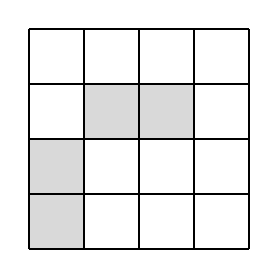
\begin{tikzpicture}[scale=0.7]
    \fill[gray!30] (0,0) rectangle (1,2);
    \fill[gray!30] (1,2) rectangle (3,3);
    \draw[step=1cm, black, thick] (0,0) grid (4,4);
\end{tikzpicture}
\\
$empty$
\end{tabular}
\begin{tabular}{c}
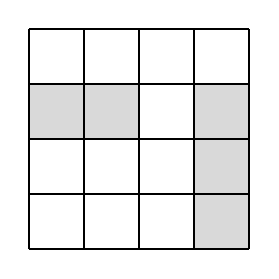
\begin{tikzpicture}[scale=0.7]
    \fill[gray!30] (0,2) rectangle (2,3);
    \fill[gray!30] (3,0) rectangle (4,3);
    \draw[step=1cm, black, thick] (0,0) grid (4,4);
\end{tikzpicture}
\\
$empty \gg 1$
\end{tabular}
\begin{tabular}{c}
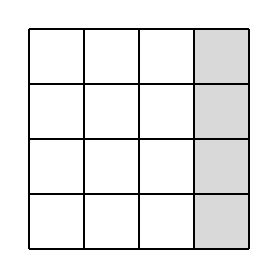
\begin{tikzpicture}[scale=0.7]
    \fill[gray!30] (3,0) rectangle (4,4);
    \draw[step=1cm, black, thick] (0,0) grid (4,4);
\end{tikzpicture}
\\
$\lnot last$
\end{tabular}
\begin{tabular}{c}
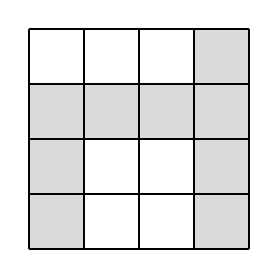
\begin{tikzpicture}[scale=0.7]
    \fill[gray!30] (0,0) rectangle (1,2);
    \fill[gray!30] (1,2) rectangle (3,3);
    \fill[gray!30] (0,2) rectangle (2,3);
    \fill[gray!30] (3,0) rectangle (4,3);
    \fill[gray!30] (3,0) rectangle (4,4);
    \draw[step=1cm, black, thick] (0,0) grid (4,4);
\end{tikzpicture}
\\
$anchors$
\end{tabular}
\\
\end{tabular}
\caption{Iskanje vodoravnih potez z bitnimi operacijami. (Siva polja predstavljajo bitne $0$, bela polja pa bitne $1$.)}
\end{figure}